\documentclass[12pt]{article}
\usepackage[utf8]{inputenc}
\usepackage{amsmath, amssymb}
\usepackage{xcolor}
\usepackage{geometry}
\usepackage{hyperref}
\usepackage{fancyhdr}
\usepackage{enumitem}
\usepackage{minted} % Code highlighting
\usepackage{booktabs} % Clean tables
\usepackage{tikz}
\usetikzlibrary{shapes, arrows, positioning, automata, calc}

\geometry{margin=1in}
\hypersetup{colorlinks=true, linkcolor=blue, urlcolor=cyan}

\pagestyle{fancy}
\fancyhf{}
\fancyhead[L]{\textbf{\TOPICTITLE}}
\fancyhead[R]{\thepage}

% -------------------------------
% Topic Metadata
% -------------------------------
\newcommand{\TOPICTITLE}{Principles of Congestion Control}
\title{\TOPICTITLE\\\large Study-Ready Notes}
\author{Compiled by Andrew Photinakis}
\date{\today}

\setlength{\headheight}{15pt}

\begin{document}
\maketitle
\tableofcontents
\newpage

% This LaTeX file should be saved at: computer_networks/transport_layer/principles_congestion_control.tex

\section{Introduction to Congestion Control}

\begin{itemize}
    \item Fundamental problem in computer networks
    \item Different from flow control (which handles sender-receiver speed mismatch)
    \item Considered one of the top-10 problems in networking
    \item Essential for network stability and fair resource sharing
\end{itemize}

\subsection{Definition and Manifestations}
\begin{itemize}
    \item \textbf{Congestion}: "Too many sources sending too much data too fast for \textit{network} to handle"
    \item \textbf{Manifestations}:
    \begin{itemize}
        \item Long delays (queueing in router buffers)
        \item Packet loss (buffer overflow at routers)
    \end{itemize}
\end{itemize}

\subsection{Congestion Control vs Flow Control}
\begin{table}[h]
    \centering
    \begin{tabular}{p{0.45\textwidth}p{0.45\textwidth}}
        \toprule
        \textbf{Congestion Control} & \textbf{Flow Control} \\
        \midrule
        Too many senders, sending too fast & One sender too fast for one receiver \\
        Network-wide problem & End-to-end problem \\
        Prevents network collapse & Prevents receiver buffer overflow \\
        Affects all users sharing network & Affects single connection \\
        \textbf{Example}: TCP congestion control & \textbf{Example}: TCP flow control (rwnd) \\
        \bottomrule
    \end{tabular}
    \caption{Comparison of congestion control vs flow control}
    \label{tab:congestion_vs_flow}
\end{table}

\textcolor{blue}{[Summary: Congestion control manages network-wide resource overutilization when too many senders overload network capacity, while flow control handles speed mismatches between individual sender-receiver pairs.]}

\section{Causes and Costs of Congestion: Three Scenarios}

\subsection{Scenario 1: Infinite Buffers, No Retransmissions}

\subsubsection{Setup}
\begin{itemize}
    \item Two flows sharing one router
    \item Infinite buffers at router
    \item Input/output link capacity: R
    \item No retransmissions needed (perfect channel)
\end{itemize}

\begin{figure}[h]
    \centering
    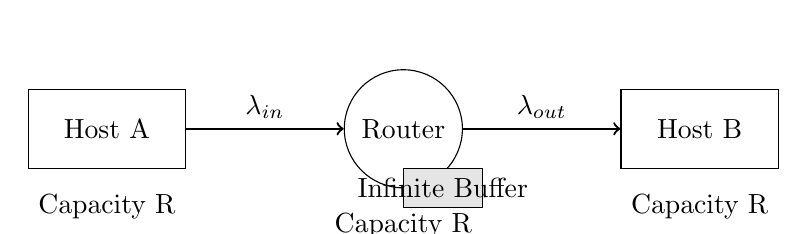
\begin{tikzpicture}[
        node distance=2cm,
        host/.style={rectangle, draw, minimum width=2cm, minimum height=1cm},
        router/.style={circle, draw, minimum size=1.5cm}
    ]
        \node[host] (hostA) {Host A};
        \node[router, right=2cm of hostA] (router) {Router};
        \node[host, right=2cm of router] (hostB) {Host B};
        
        % Links
        \draw[->, thick] (hostA) -- node[above] {$\lambda_{in}$} (router);
        \draw[->, thick] (router) -- node[above] {$\lambda_{out}$} (hostB);
        
        % Buffer
        \draw[fill=gray!20] ($(router)+(0,-1)$) rectangle ($(router)+(1,-0.5)$);
        \node at ($(router)+(0.5,-0.75)$) {Infinite Buffer};
        
        % Capacity labels
        \node[below=0.2cm of hostA] {Capacity R};
        \node[below=0.2cm of router] {Capacity R};
        \node[below=0.2cm of hostB] {Capacity R};
        
    \end{tikzpicture}
    \caption{Scenario 1: Two flows sharing router with infinite buffers}
    \label{fig:scenario1}
\end{figure}

\subsubsection{Behavior and Costs}
\begin{itemize}
    \item Maximum per-connection throughput: R/2
    \item As arrival rate $\lambda_{in}$ approaches R/2:
    \begin{itemize}
        \item Large delays due to queueing
        \item Throughput approaches R/2
        \item No packet loss (infinite buffers)
    \end{itemize}
\end{itemize}

\[
\text{Maximum throughput per connection} = \frac{R}{2}
\]

\subsection{Scenario 2: Finite Buffers with Retransmissions}

\subsubsection{Setup}
\begin{itemize}
    \item One router with finite buffers
    \item Sender retransmits lost/timed-out packets
    \item Transport-layer input includes retransmissions: $\lambda'_{in} \geq \lambda_{in}$
    \item Application-layer input = application-layer output: $\lambda_{in} = \lambda_{out}$
\end{itemize}

\begin{figure}[h]
    \centering
    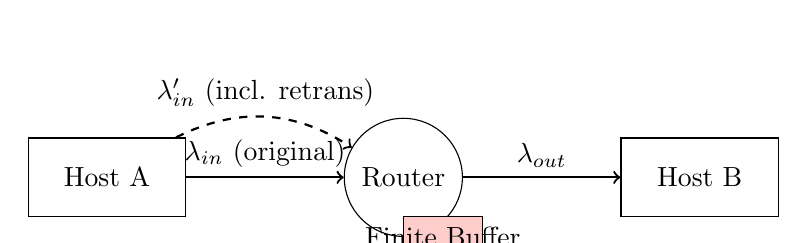
\begin{tikzpicture}[
        node distance=2cm,
        host/.style={rectangle, draw, minimum width=2cm, minimum height=1cm},
        router/.style={circle, draw, minimum size=1.5cm}
    ]
        \node[host] (hostA) {Host A};
        \node[router, right=2cm of hostA] (router) {Router};
        \node[host, right=2cm of router] (hostB) {Host B};
        
        % Data flows
        \draw[->, thick] (hostA) -- node[above] {$\lambda_{in}$ (original)} (router);
        \draw[->, thick, dashed] (hostA) to[bend left=30] node[above] {$\lambda'_{in}$ (incl. retrans)} (router);
        \draw[->, thick] (router) -- node[above] {$\lambda_{out}$} (hostB);
        
        % Finite buffer
        \draw[fill=red!20] ($(router)+(0,-1)$) rectangle ($(router)+(1,-0.5)$);
        \node at ($(router)+(0.5,-0.75)$) {Finite Buffer};
        
    \end{tikzpicture}
    \caption{Scenario 2: Finite buffers with retransmissions}
    \label{fig:scenario2}
\end{figure}

\subsubsection{Ideal Case: Perfect Knowledge}
\begin{itemize}
    \item Sender sends only when router buffers available
    \item No unneeded retransmissions
    \item Still have "wasted" capacity due to needed retransmissions
\end{itemize}

\subsubsection{Realistic Case: Unneeded Duplicates}
\begin{itemize}
    \item Premature timeouts cause unneeded duplicate transmissions
    \item Both original and duplicate copies may be delivered
    \item Further decreases effective throughput
\end{itemize}

\subsubsection{Costs in Scenario 2}
\begin{itemize}
    \item More work (retransmissions) for given receiver throughput
    \item Unneeded retransmissions waste link capacity
    \item Decreased maximum achievable throughput
\end{itemize}

\textcolor{orange}{[Mnemonic: "Finite Buffers, Infinite Problems" - Finite buffers lead to packet loss, which causes retransmissions that further congest the network.]}

\subsection{Scenario 3: Multi-Hop Paths with Multiple Senders}

\subsubsection{Setup}
\begin{itemize}
    \item Four senders with multi-hop paths
    \item Timeout/retransmit mechanisms
    \item Complex interactions between flows
\end{itemize}

\begin{figure}[h]
    \centering
    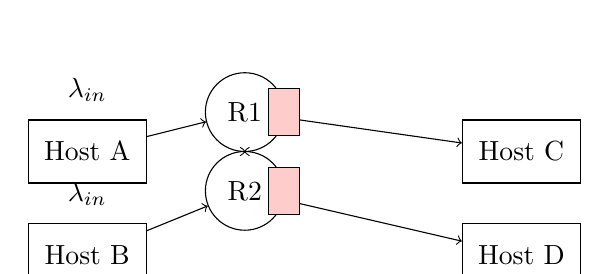
\begin{tikzpicture}[
        node distance=1.5cm,
        host/.style={rectangle, draw, minimum width=1.5cm, minimum height=0.8cm},
        router/.style={circle, draw, minimum size=1cm}
    ]
        % Hosts
        \node[host] (hostA) {Host A};
        \node[host, below=0.5cm of hostA] (hostB) {Host B};
        \node[host, right=4cm of hostA] (hostC) {Host C};
        \node[host, below=0.5cm of hostC] (hostD) {Host D};
        
        % Routers
        \node[router] (router1) at (2,0.5) {R1};
        \node[router] (router2) at (2,-0.5) {R2};
        
        % Connections
        \draw[->] (hostA) -- (router1);
        \draw[->] (hostB) -- (router2);
        \draw[->] (router1) -- (hostC);
        \draw[->] (router2) -- (hostD);
        \draw[->] (router1) -- (router2);
        \draw[->] (router2) -- (router1);
        
        % Data flows
        \node[above=0.1cm of hostA] {$\lambda_{in}$};
        \node[above=0.1cm of hostB] {$\lambda_{in}$};
        
        % Buffer indication
        \draw[fill=red!20] ($(router1)+(0.3,-0.3)$) rectangle ($(router1)+(0.7,0.3)$);
        \draw[fill=red!20] ($(router2)+(0.3,-0.3)$) rectangle ($(router2)+(0.7,0.3)$);
        
    \end{tikzpicture}
    \caption{Scenario 3: Multiple senders with multi-hop paths}
    \label{fig:scenario3}
\end{figure}

\subsubsection{Critical Insight}
\begin{itemize}
    \item As red $\lambda'_{in}$ increases, all arriving blue packets at upper queue are dropped
    \item Blue throughput approaches zero due to congestion collapse
    \item Upstream transmission capacity and buffering wasted for packets lost downstream
\end{itemize}

\subsection{Summary of Congestion Costs}
\begin{itemize}
    \item Throughput can never exceed capacity
    \item Delay increases as capacity approached
    \item Loss/retransmission decreases effective throughput
    \item Unneeded duplicates further decrease effective throughput
    \item Upstream resources wasted for packets lost downstream
    \item Potential for congestion collapse (throughput → 0)
\end{itemize}

\textcolor{blue}{[Summary: Congestion costs include decreased throughput, increased delay, wasted resources on retransmissions, and potential congestion collapse where useful throughput drops to near zero despite high network load.]}

\section{Approaches to Congestion Control}

\subsection{End-to-End Congestion Control}

\begin{itemize}
    \item No explicit feedback from network
    \item Congestion \textit{inferred} from observed loss and delay
    \item Approach taken by standard TCP
    \item Senders monitor ACK patterns and timing
\end{itemize}

\begin{figure}[h]
    \centering
    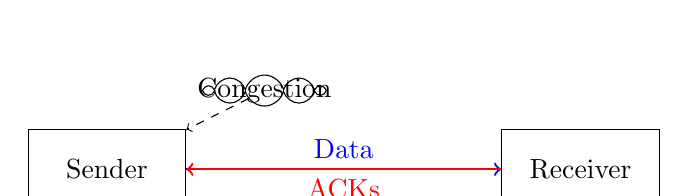
\begin{tikzpicture}[
        node distance=2cm,
        host/.style={rectangle, draw, minimum width=2cm, minimum height=1cm}
    ]
        \node[host] (sender) {Sender};
        \node[host, right=4cm of sender] (receiver) {Receiver};
        
        % Data and ACK flow
        \draw[->, thick, blue] (sender) -- node[above] {Data} (receiver);
        \draw[->, thick, red] (receiver) -- node[below] {ACKs} (sender);
        
        % Congestion inference
        \node[draw, cloud, cloud puffs=10, cloud ignores aspect, minimum width=1.5cm] (congestion) at (2,1) {};
        \node at (2,1) {Congestion};
        
        \draw[->, dashed] (congestion) -- (sender);
        
    \end{tikzpicture}
    \caption{End-to-end congestion control: sender infers congestion from ACK patterns}
    \label{fig:end_to_end}
\end{figure}

\subsection{Network-Assisted Congestion Control}

\begin{itemize}
    \item Routers provide direct feedback to sending/receiving hosts
    \item May indicate congestion level or explicitly set sending rate
    \item More explicit and potentially faster response
\end{itemize}

\begin{table}[h]
    \centering
    \begin{tabular}{p{0.45\textwidth}p{0.45\textwidth}}
        \toprule
        \textbf{End-to-End Control} & \textbf{Network-Assisted Control} \\
        \midrule
        Congestion inferred from loss/delay & Explicit feedback from routers \\
        Implemented at transport layer & Requires router participation \\
        TCP standard approach & TCP ECN, ATM, DECbit \\
        Slower to react & Faster, more precise reaction \\
        Works with existing infrastructure & Requires router upgrades \\
        \textbf{Advantage}: Deployment ease & \textbf{Advantage}: Performance \\
        \bottomrule
    \end{tabular}
    \caption{Comparison of end-to-end vs network-assisted congestion control}
    \label{tab:control_approaches}
\end{table}

\subsection{Examples of Network-Assisted Approaches}
\begin{itemize}
    \item \textbf{TCP ECN (Explicit Congestion Notification)}: Routers mark packets to indicate congestion
    \item \textbf{ATM (Asynchronous Transfer Mode)}: Complex signaling for congestion control
    \item \textbf{DECbit}: Early research protocol using single bit for congestion indication
\end{itemize}

\begin{figure}[h]
    \centering
    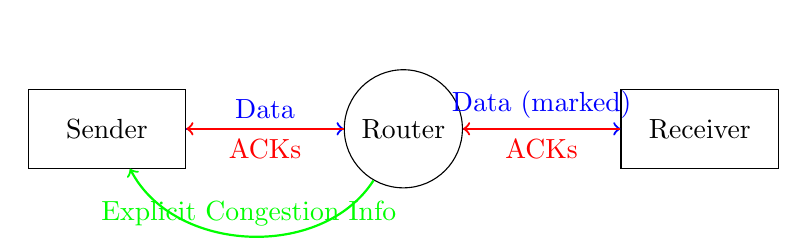
\begin{tikzpicture}[
        node distance=2cm,
        host/.style={rectangle, draw, minimum width=2cm, minimum height=1cm},
        router/.style={circle, draw, minimum size=1.5cm}
    ]
        \node[host] (sender) {Sender};
        \node[router, right=2cm of sender] (router) {Router};
        \node[host, right=2cm of router] (receiver) {Receiver};
        
        % Data flow with congestion marking
        \draw[->, thick, blue] (sender) -- node[above] {Data} (router);
        \draw[->, thick, blue] (router) -- node[above] {Data (marked)} (receiver);
        
        % ACK flow
        \draw[->, thick, red] (receiver) -- node[below] {ACKs} (router);
        \draw[->, thick, red] (router) -- node[below] {ACKs} (sender);
        
        % Explicit congestion info
        \draw[->, thick, green] (router) to[bend left=60] node[above] {Explicit Congestion Info} (sender);
        
    \end{tikzpicture}
    \caption{Network-assisted congestion control: routers provide explicit feedback}
    \label{fig:network_assisted}
\end{figure}

\textcolor{teal}{[Concept Map: Congestion Control Approaches → End-to-End (TCP: infer from loss/delay) vs Network-Assisted (ECN, ATM: explicit feedback) → Trade-off between deployment ease and performance → Both aim to prevent congestion collapse and ensure fair resource sharing.]}

\section{Congestion Control Insights and Principles}

\subsection{Fundamental Trade-offs}
\begin{itemize}
    \item \textbf{Fairness vs Efficiency}: Maximizing total throughput may not be fair to all users
    \item \textbf{Responsiveness vs Stability}: Quick reaction vs oscillation prevention
    \item \textbf{Simplicity vs Optimality}: Easy implementation vs perfect performance
\end{itemize}

\subsection{Key Design Principles}
\begin{enumerate}
    \item \textbf{Conserve Packets}: Don't send unless network can deliver
    \item \textbf{Adapt to Change}: Adjust rates based on network conditions
    \item \textbf{Distribute Fairly}: All flows should get reasonable share
    \item \textbf{Avoid Collapse}: Prevent throughput dropping to zero
    \item \textbf{Scale Well}: Work in networks of all sizes
\end{enumerate}

\subsection{Mathematical Foundations}
The relationship between offered load and achieved throughput can be modeled as:

\[
\text{Effective Throughput} = \frac{\text{Offered Load}}{1 + \text{Retransmission Overhead}}
\]

Where retransmission overhead increases non-linearly with offered load.

\begin{figure}[h]
    \centering
    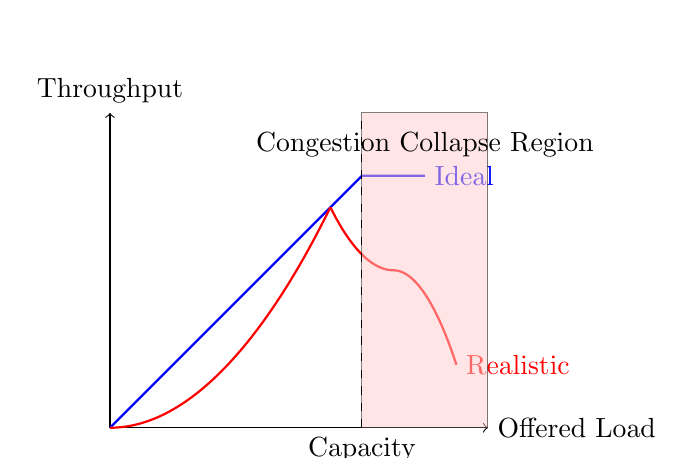
\begin{tikzpicture}[scale=0.8]
        \draw[->] (0,0) -- (6,0) node[right] {Offered Load};
        \draw[->] (0,0) -- (0,5) node[above] {Throughput};
        
        % Ideal line
        \draw[thick, blue] (0,0) -- (4,4) -- (5,4);
        \node[blue, right] at (5,4) {Ideal};
        
        % Realistic curve
        \draw[thick, red] (0,0) parabola (3.5,3.5);
        \draw[thick, red] (3.5,3.5) parabola bend (4.5,2.5) (5.5,1);
        \node[red, right] at (5.5,1) {Realistic};
        
        % Congestion collapse region
        \draw[fill=red!20, opacity=0.5] (4,0) rectangle (6,5);
        \node at (5,4.5) {Congestion Collapse Region};
        
        \draw[dashed] (4,0) -- (4,5);
        \node[below] at (4,0) {Capacity};
        
    \end{tikzpicture}
    \caption{Relationship between offered load and throughput showing congestion collapse}
    \label{fig:throughput_curve}
\end{figure}

\textcolor{blue}{[Summary: Effective congestion control must balance fairness, efficiency, and stability while preventing congestion collapse, using either end-to-end inference or network-assisted explicit feedback mechanisms.]}

\section{Study Aids and Exam Preparation}

\subsection{Key Concepts to Master}
\begin{itemize}
    \item Understand the three congestion scenarios and their specific costs
    \item Differentiate between congestion control and flow control
    \item Compare end-to-end vs network-assisted approaches
    \item Explain the causes of congestion collapse
    \item Describe the trade-offs in congestion control design
\end{itemize}

\subsection{Practice Questions}
\begin{enumerate}
    \item \textbf{Compare and contrast} the three congestion scenarios discussed. What specific costs does each scenario illustrate, and how do they build upon each other?
    
    \item Explain why \textbf{congestion control} is fundamentally different from \textbf{flow control}. Provide concrete examples of each and describe what problems they solve.
    
    \item Describe the \textbf{congestion collapse} phenomenon. How can it occur in Scenario 3, and what mechanisms can prevent it?
    
    \item Compare \textbf{end-to-end congestion control} with \textbf{network-assisted congestion control}. What are the advantages and disadvantages of each approach?
    
    \item A network has a bottleneck link with capacity R. If N TCP connections share this link fairly, what is the maximum throughput each can achieve? What happens as N becomes very large?
\end{enumerate}

\textcolor{orange}{[Mnemonic: "End-to-End Estimates, Network Notifies" - End-to-end control estimates congestion from observations, while network-assisted control provides explicit notifications.]}

\section{Summary}

\begin{itemize}
    \item Congestion occurs when network resources are overutilized by too many senders
    \item Three scenarios illustrate progressive complexity of congestion costs:
    \begin{itemize}
        \item Scenario 1: Delay increases with infinite buffers
        \item Scenario 2: Retransmissions waste capacity with finite buffers
        \item Scenario 3: Congestion collapse possible in multi-hop networks
    \end{itemize}
    \item Costs include decreased throughput, increased delay, and wasted resources
    \item Two main approaches:
    \begin{itemize}
        \item End-to-end control (TCP standard): Infer congestion from observations
        \item Network-assisted control (ECN, ATM): Explicit router feedback
    \end{itemize}
    \item Effective congestion control must balance fairness, efficiency, and stability
    \item Prevention of congestion collapse is critical for network operation
\end{itemize}

\section{References}
\begin{itemize}
    \item Kurose, J.F., \& Ross, K.W. (2020). \textit{Computer Networking: A Top-Down Approach (8th ed.)}. Pearson.
    \item Course: COMPSCI 453 Computer Networks, University of Massachusetts
    \item Professor: Jim Kurose, College of Information and Computer Sciences
    \item Jacobson, V. (1988). "Congestion Avoidance and Control"
    \item RFC 5681: TCP Congestion Control
    \item Textbook website: http://gala.cs.umass.edu/kurose\_ross
\end{itemize}

\end{document}